Bien qu'un peu longue à rédiger, la preuve présentée ici est presque évidente par simple lecture des dessins bien codés ci-après. En tout cas, elle s'explique très vite à l'oral sans faire appel à aucun calcul !


\bigskip


\textbf{Cas 1.} \emph{Supposons que $A = I$ ou $B = I$ .}

\medskip

Par symétrie des rôles, on peut juste traiter la situation où $A = I$ . Dans ce cas, $\vangleorient{OI}{OA}$ est nul d'où $\vangleorient{OI}{OS} = \vangleorient{OI}{OB}$ soit $B = S$ . On conclut comme suit.

\begin{enumerate}
	\item Si $A \neq B$ alors la parallèle à $(AB)$ passant par $I = A$ n'est autre que $(AB)$ .
	Suivant que cette parallèle est tangente ou non au cercle, on aura bien à chaque fois $S = B$ .

	\item Si $A = B$ , on raisonne de même avec la parallèle à la tangente en $A$ au cercle.
\end{enumerate}


% -------------- %


\bigskip


\textbf{Cas 2.} \emph{Supposons que $A \neq B$ avec $A \neq I$ et $B \neq I$ .}

\medskip

Nous avons donc une situation du type suivant où sont indiqués des angles très intéressants comme nous allons le constater tout de suite.

\smallskip
\begin{center}
	\fbox{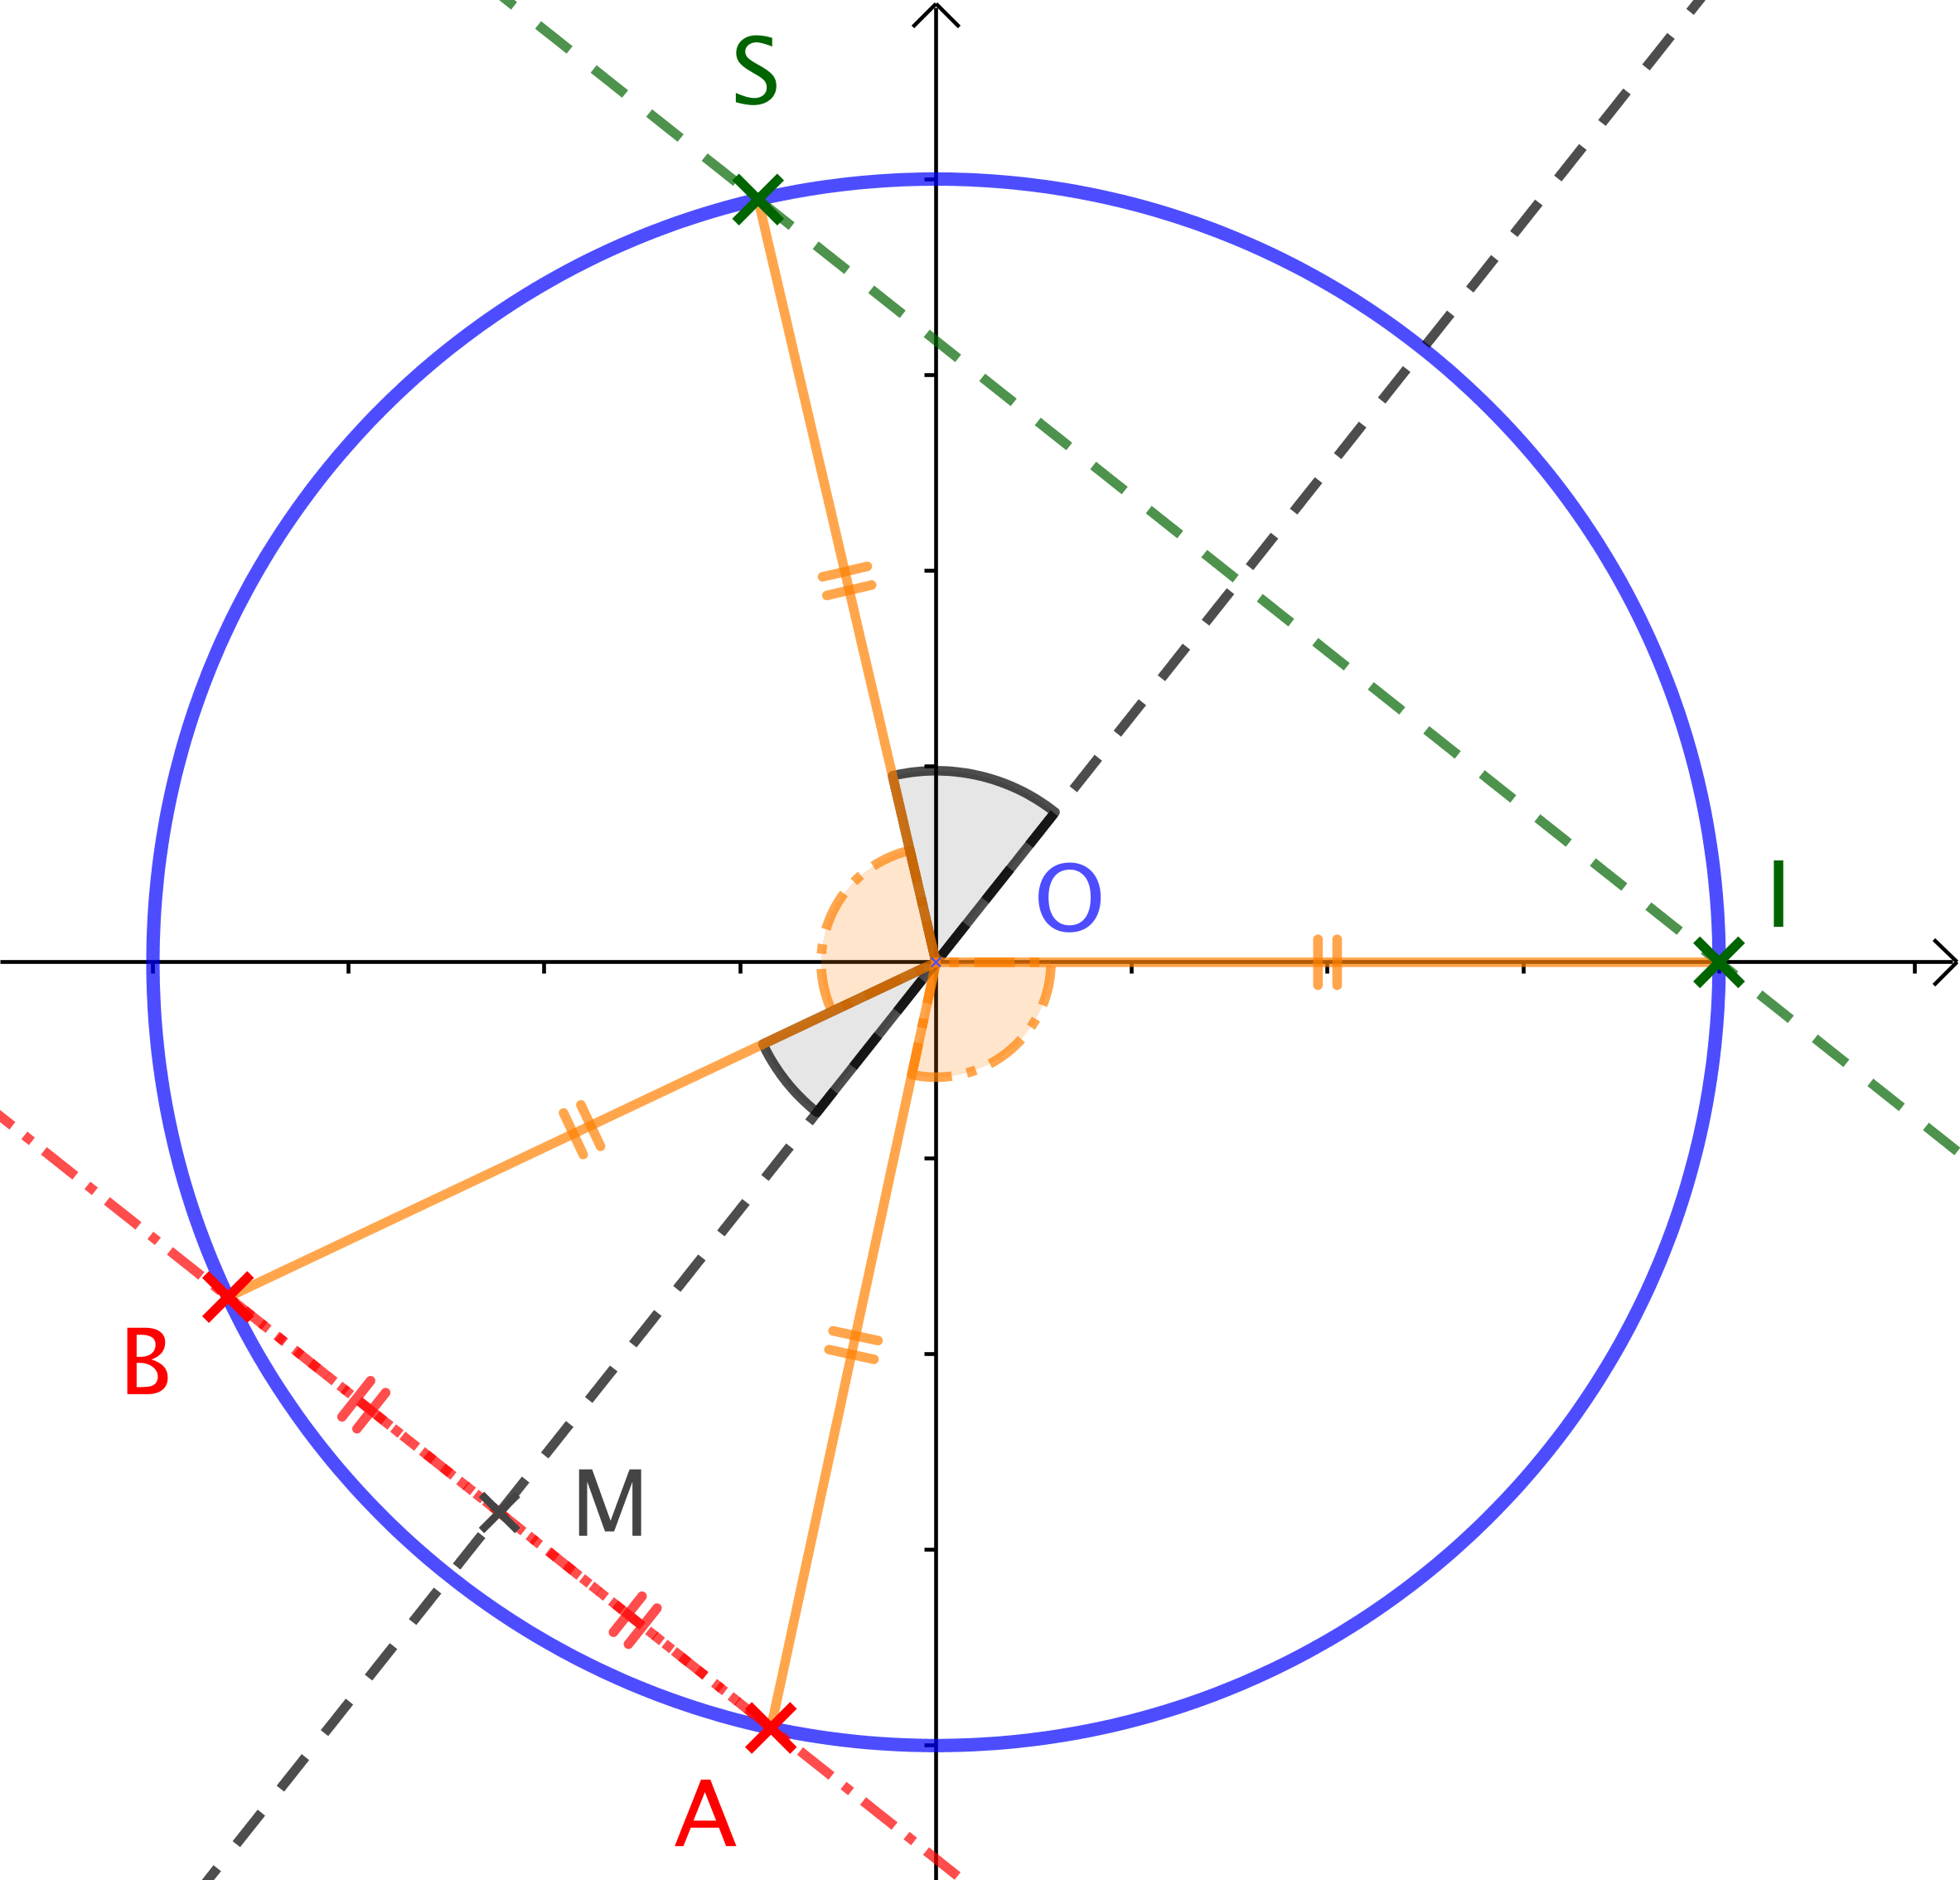
\includegraphics[scale = .75]{addition-on-ellipsis/proof/rotation-A-not-B.png}}
\end{center}
\smallskip

Comme 
$\angleorient{\vect{OB}}{\vect{OS}}
= \angleorient{\vect{OB}}{\vect{OI}}
+ \angleorient{\vect{OI}}{\vect{OS}}$
et
$\angleorient{\vect{OI}}{\vect{OS}}
= \angleorient{\vect{OI}}{\vect{OA}}
+ \angleorient{\vect{OI}}{\vect{OB}}$ 
par définition de $S$ , nous avons :
$\angleorient{\vect{OB}}{\vect{OS}}
= \angleorient{\vect{OI}}{\vect{OA}}$
.


\smallskip

Ensuite, notant $M$ le milieu de $[AB]$ , la médiane $(OM)$ est aussi une bissectrice du triangle $BOA$ isocèle en $O$ de sorte que
$\angleorient{\vect{OM}}{\vect{OB}} 
= - \angleorient{\vect{OM}}{\vect{OA}}$ 
.


\smallskip

Notant $\Pi$ l'angle plat, nous avons alors :
\begin{flalign*}
	\angleorient{\vect{MO}}{\vect{OS}}
		&= \angleorient{\vect{MO}}{\vect{OM}} 
		 + \angleorient{\vect{OM}}{\vect{OB}}
		 + \angleorient{\vect{OB}}{\vect{OS}}
		& \\
		&= \Pi
		 - \angleorient{\vect{OM}}{\vect{OA}}
		 + \angleorient{\vect{OI}}{\vect{OA}}
		& \\
		&= \Pi
		 + \angleorient{\vect{OA}}{\vect{OM}}
		 + \angleorient{\vect{OI}}{\vect{OA}}
		& \\
		&= \Pi
		 + \angleorient{\vect{OI}}{\vect{OM}}
		& \\
		&= \angleorient{\vect{OI}}{- \, \vect{OM}}
		& \\
		&= \angleorient{\vect{OI}}{\vect{MO}}
		& \\
		&= - \angleorient{\vect{MO}}{\vect{OI}}
		& \\
\end{flalign*}

\vspace{-1.5em}


Comme
$\angleorient{\vect{MO}}{\vect{OS}} 
= - \angleorient{\vect{MO}}{\vect{OI}}$ ,
la droite $(OM)$ est aussi une bissectrice du triangle $SOI$ isocèle en $O$ .
Or la bissectrice issue du sommet principal d'un triangle isocèle est aussi une hauteur d'où $(OM) \,\bot\, (AB)$ et $(OM) \,\bot\, (SI)$ puis $(AB) \,/\!/\, (SI)$ comme souhaité.



% -------------- %


\bigskip

\textbf{Cas 3.} \emph{Supposons que $A = B \neq I$ .}

\medskip

Tout est dans le dessin suivant ou presque. Nous allons rédiger cela proprement.

\smallskip
\begin{center}
	\fbox{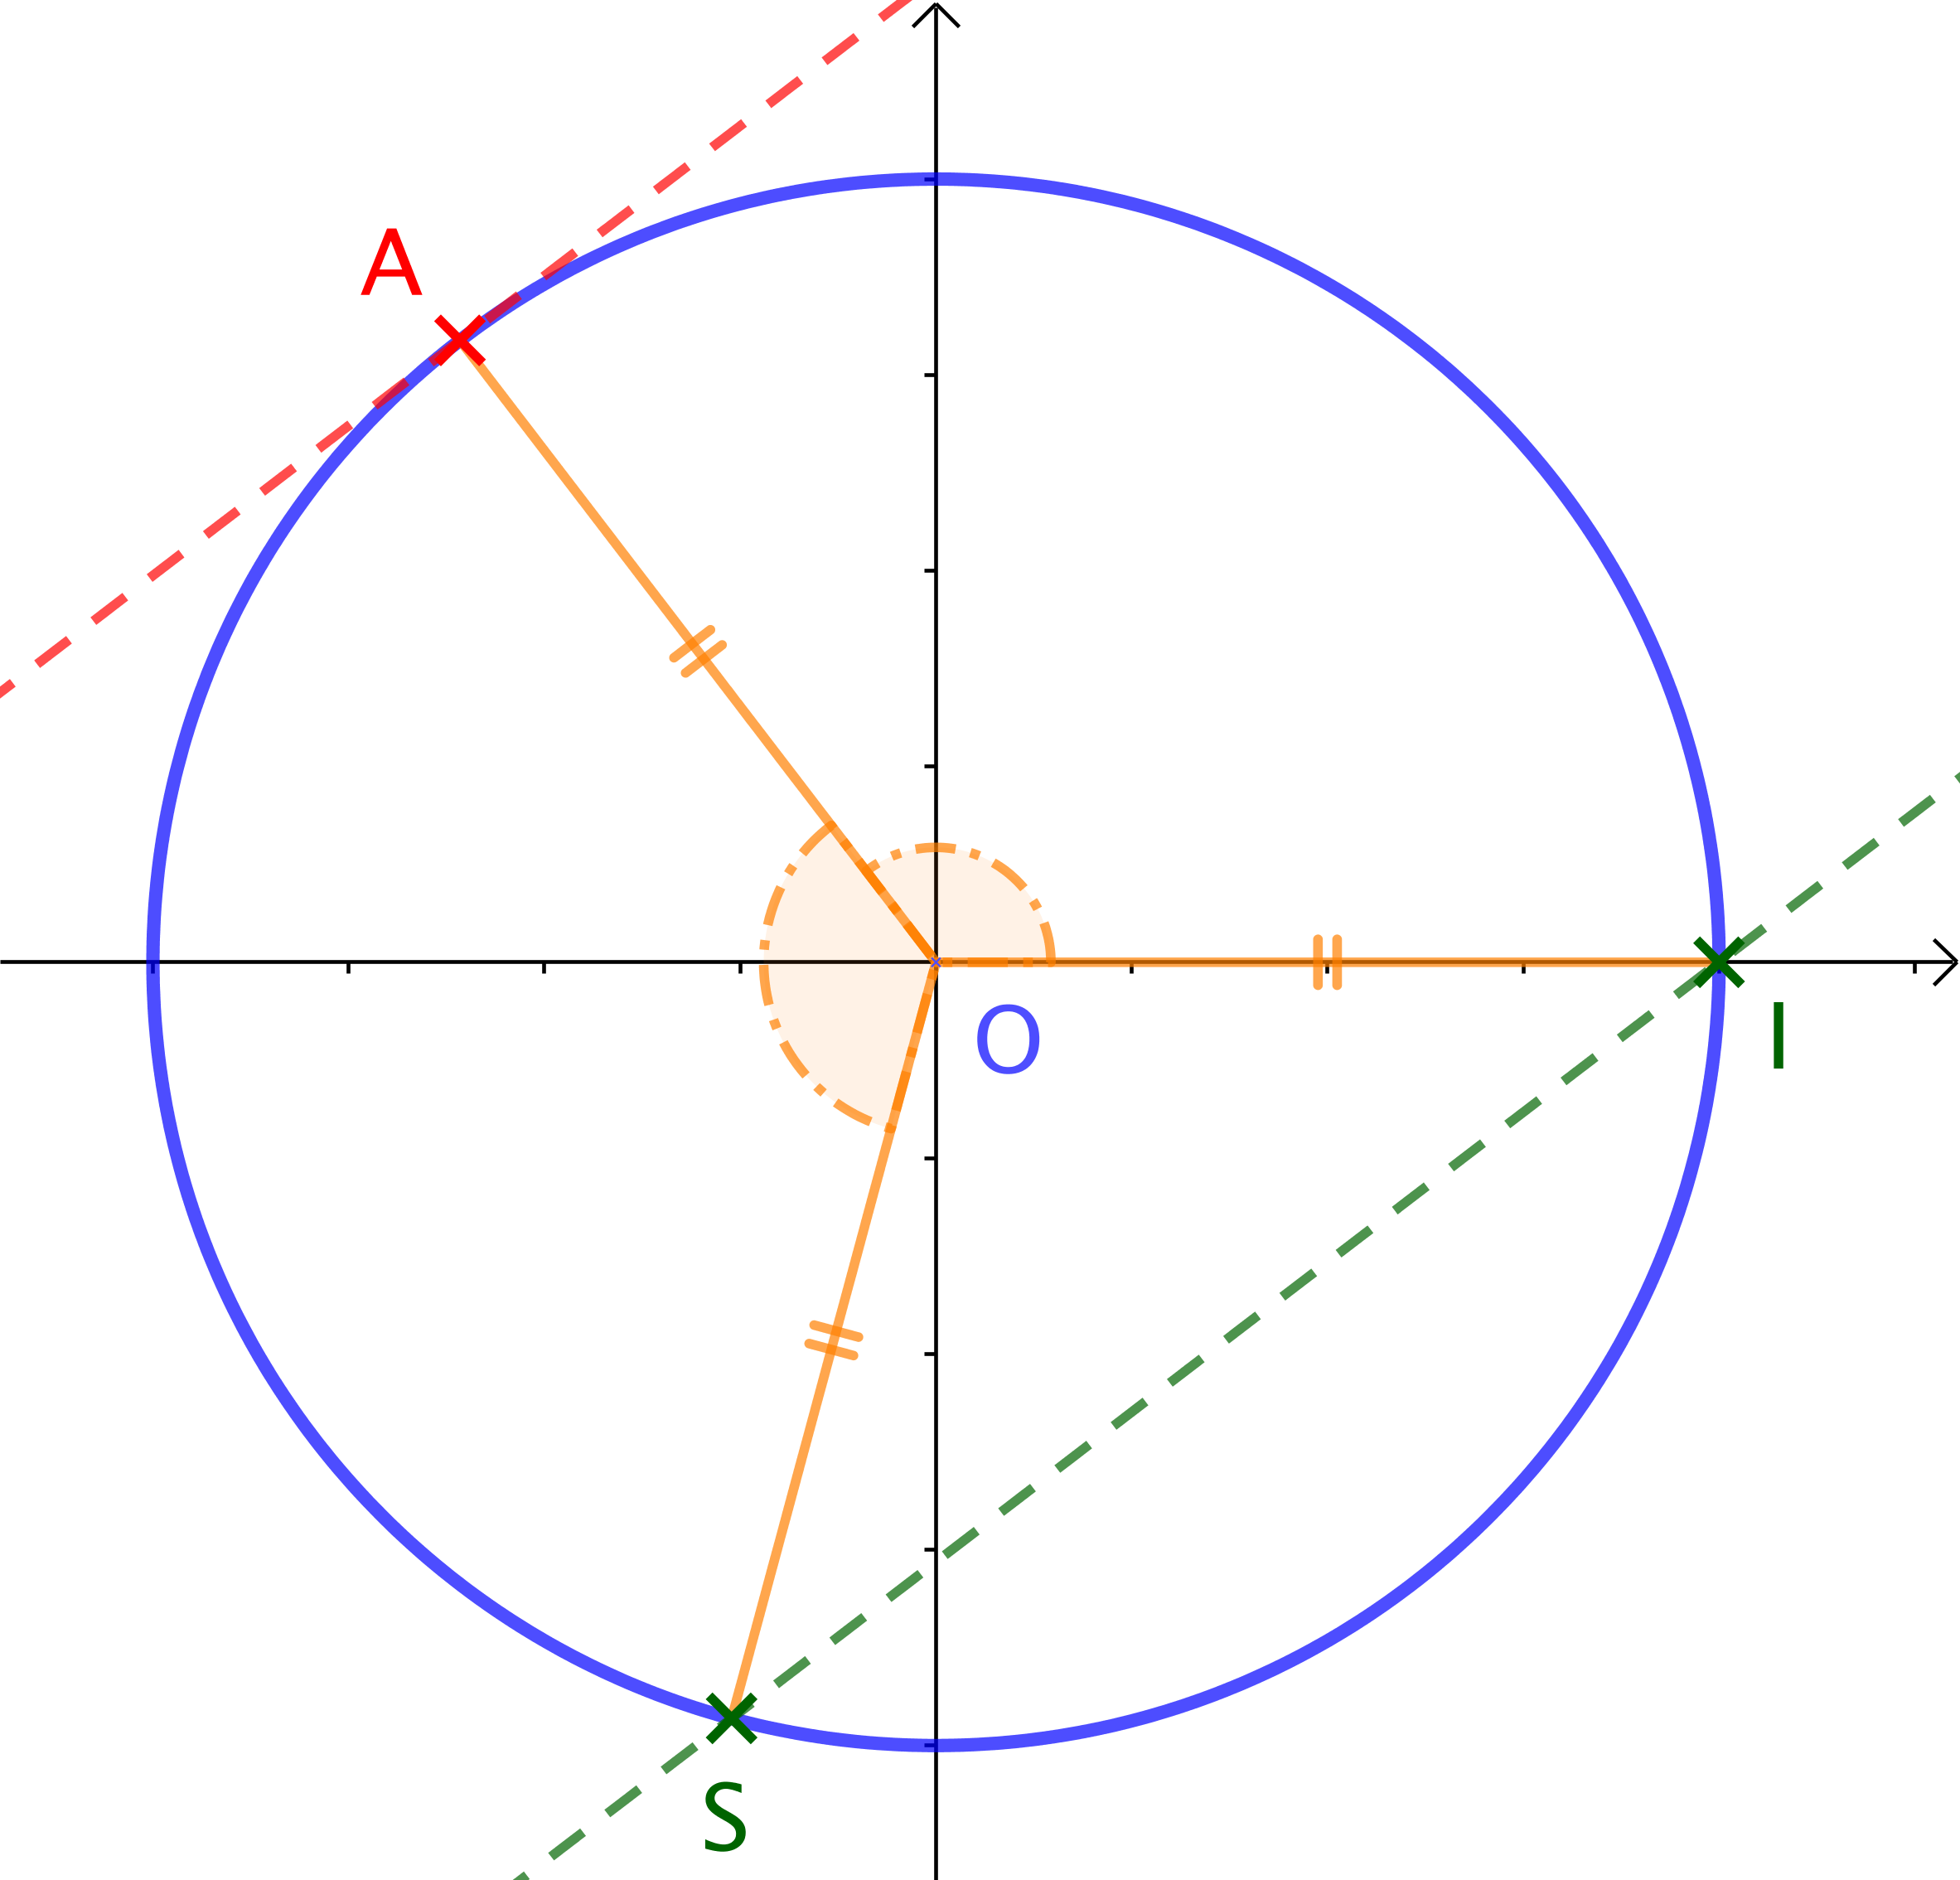
\includegraphics[scale = .75]{addition-on-ellipsis/proof/rotation-A-is-B.png}}
\end{center}
\smallskip

Il est immédiat que
$\angleorient{\vect{OI}}{\vect{OA}}
= \angleorient{\vect{OA}}{\vect{OS}}$
puis que
$- \angleorient{\vect{AO}}{\vect{OI}}
= \angleorient{\vect{AO}}{\vect{OS}}$ .
Nous en déduisons que la droite $(AO)$ est la bissectrice du triangle isocèle $SOI$  issue du sommet principal de ce dernier d'où $(AO) \,\bot\, (SI)$ puisque cette bissectrice particulière est aussi une hauteur. Il est alors clair que $(SI)$ est parallèle à la tangente en $A$ au cercle.
